\nsection{Problem 5 - (Stochastic gradient decent, SGD)}
In this exercise we will try out the minibatch approach for optimizing neural nets. We will consider a simple 1D situation. The input $x$ and output $y$ are both one dimensional. We will use a model architecture with one hidden layer, and a width of 50. As the activation function, $\sigma(x)$, you should use the $\mathrm{ReLu}$, which is defined as:
$$
\sigma(x)=\left\{\begin{array}{l}
x \text { for } x>0 \\
0 \text { for } x \leq 0
\end{array}\right.
$$

Define also the derivative of the activation function to be:
$$
\sigma^{\prime}(x)=\left\{\begin{array}{l}
1 \text { for } x>0 \\
0 \text { for } x \leq 0
\end{array}\right.
$$

The estimator have the form (also called the architecture):
$$
f(x)=\sum_{i=1}^{50} \beta_i \sigma\left(\alpha_i x_i +\alpha_{0, i}\right)+\beta_0
$$
We will minimize the squared sum of errors:
$$
\text { sse }=\sum_{i=1}^N\left(y_i-\hat{f}\left(x_i\right)\right)^2
$$
\nssection{a.)}
\emph{Adapt the formulas from the lecture slides or the SGD note of Geir Storvik such that
these can be used for the specific problem formulation defined above. Present the
formulas that are relevant for implementing SGD on the current problem. How many
parameters are there in the architecture?} \spaze
\textbf{Solution:} \spaze
When dealing with neural networks, it is crucial to optimize the magnitude of the cost or loss function associated with the architecture. This optimization process involves constructing and examining the backpropagation steps, which are responsible for training our model. Backpropagation essentially estimates the parameters of interest in the given model derived from the information of the gradient. This in turn tells us how we should update the parameters. \spaze
By this reasoning we proceed to calculate the gradient of our cost function 
\begin{align*}
    \mathcal{C}(\theta) = \text{sse} = \sum_{i=1}^N\left(y_i-\hat{f}\left(x_i\right)\right)^2
\end{align*}
with respect to all influential parameters $\beta_0, \beta_i, \alpha_i, \alpha_{0,i}$. This yields 
\begin{align}
    \frac{\partial}{\partial \beta_0} \mathcal{C}(\theta) &= -2 \sum_{i=1}^N (y_i - f(x_i)) \\[7pt]
     \frac{\partial}{\partial \beta_i} \mathcal{C}(\theta) &= -2 \sum_{i=1}^N \left( y_i -  f(x_i) \right) \sigma\left(\alpha_i x+\alpha_{0, i}\right) \\[7pt]
    \frac{\partial}{\partial \alpha_i} \mathcal{C}(\theta) &= -2 \sum_{i=1}^N \left( y_i -  f(x_i) \right)\beta_i \sigma^{\prime} \left(\alpha_i x+\alpha_{0, i}\right)x_i \\[7pt]
    \frac{\partial}{\partial \alpha_{0,i}} \mathcal{C}(\theta) &= -2 \sum_{i=1}^N \left( y_i -  f(x_i) \right)\beta_i \sigma^{\prime} \left(\alpha_i x+\alpha_{0, i}\right).
\end{align}
Since we are presented with a network of $N = 50$ nodes there are hence 50 values of $\beta_i$, 50 $\alpha_i$, 50 $\alpha_{0,1}$ and additionally a singular $\beta_0$, giving $50 + 50 + 50 + 1 = 151$ parameters. 
\nssection{b.)}
\emph{Implement the SGD for the architecture above and test it on the data found in}
\texttt{functionEstimationNN.dat} 
\emph{Test different alternatives for the learning rate and
record the test error for each epoch. Use a batch size of 50.} \spaze
\textbf{Solution:} \spaze
The code of the implementation can be found in Appendix \ref{appendix:b}, from code lisitings (\ref{lst:sgd}) and produces the following plots 
\begin{figure}[H]
\centering
\begin{subfigure}{0.32\textwidth}
  \centering
  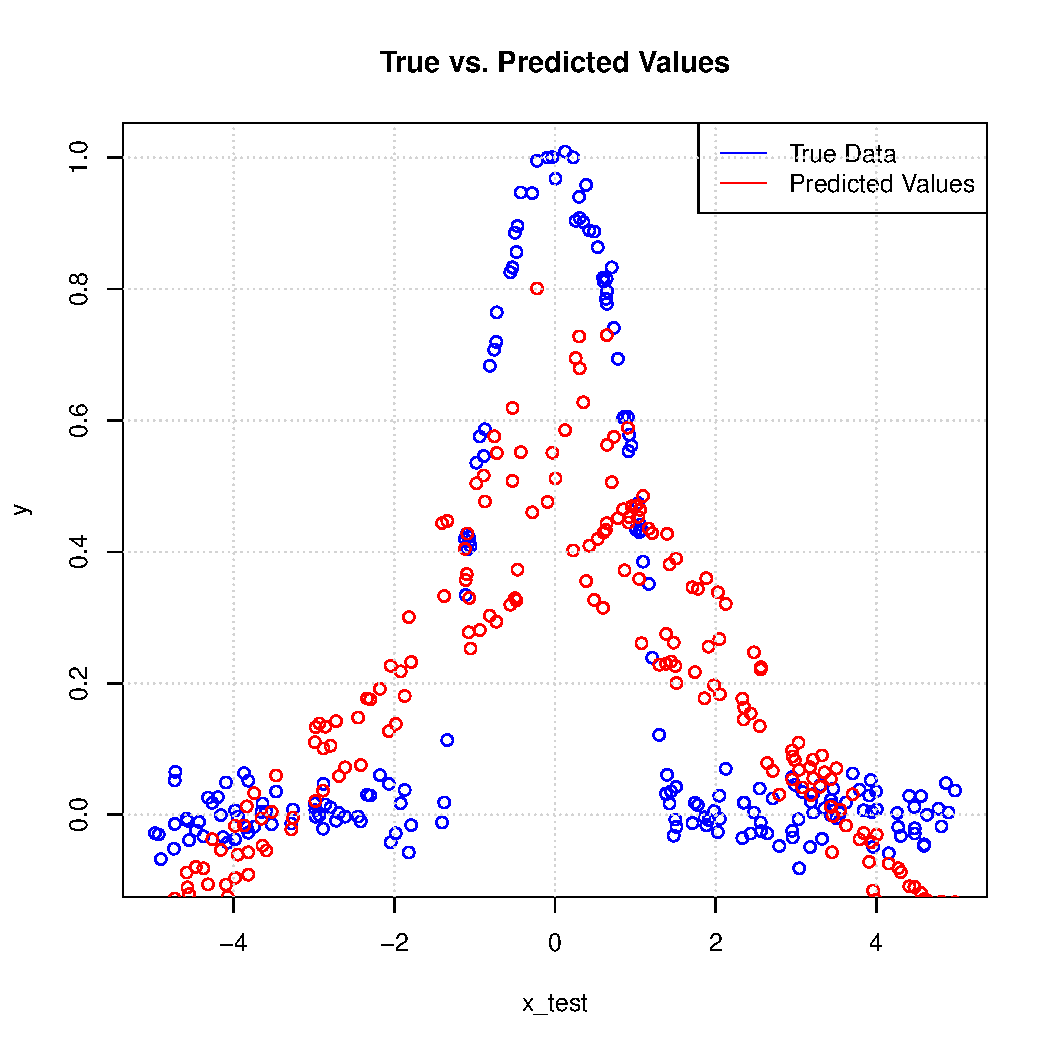
\includegraphics[width=\linewidth]{Images/Figures_Exercise_5/True_v_Predict.pdf} 
  \caption{Point plot, True vs Predicted}
  \label{fig:point_pred_true}
\end{subfigure}
\hfill
\begin{subfigure}{0.32\textwidth}
  \centering
  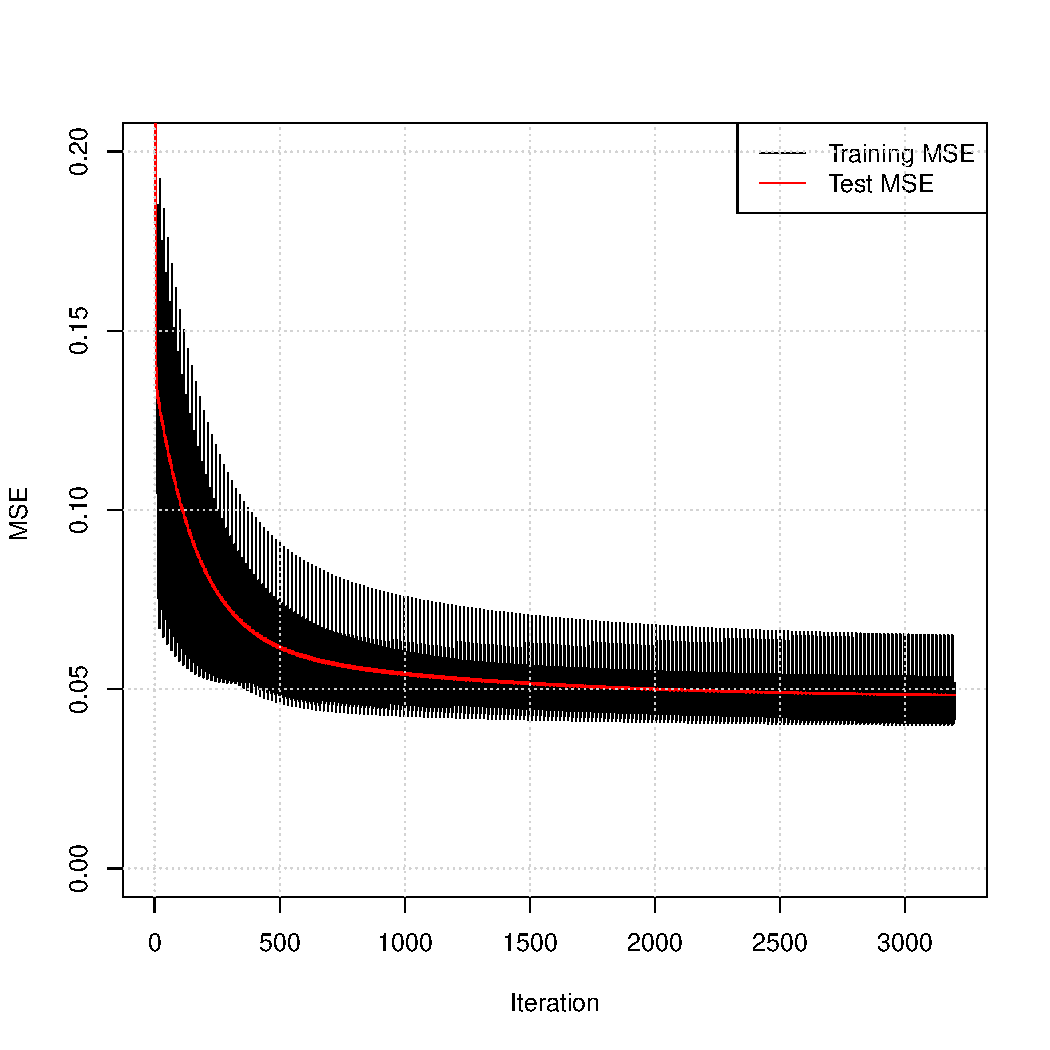
\includegraphics[width=\linewidth]{Images/Figures_Exercise_5/MSE_train_test.pdf} 
  \caption{Evolution of MSE}
  \label{fig:MSE_evol}
\end{subfigure}
\hfill
\begin{subfigure}{0.32\textwidth}
  \centering
  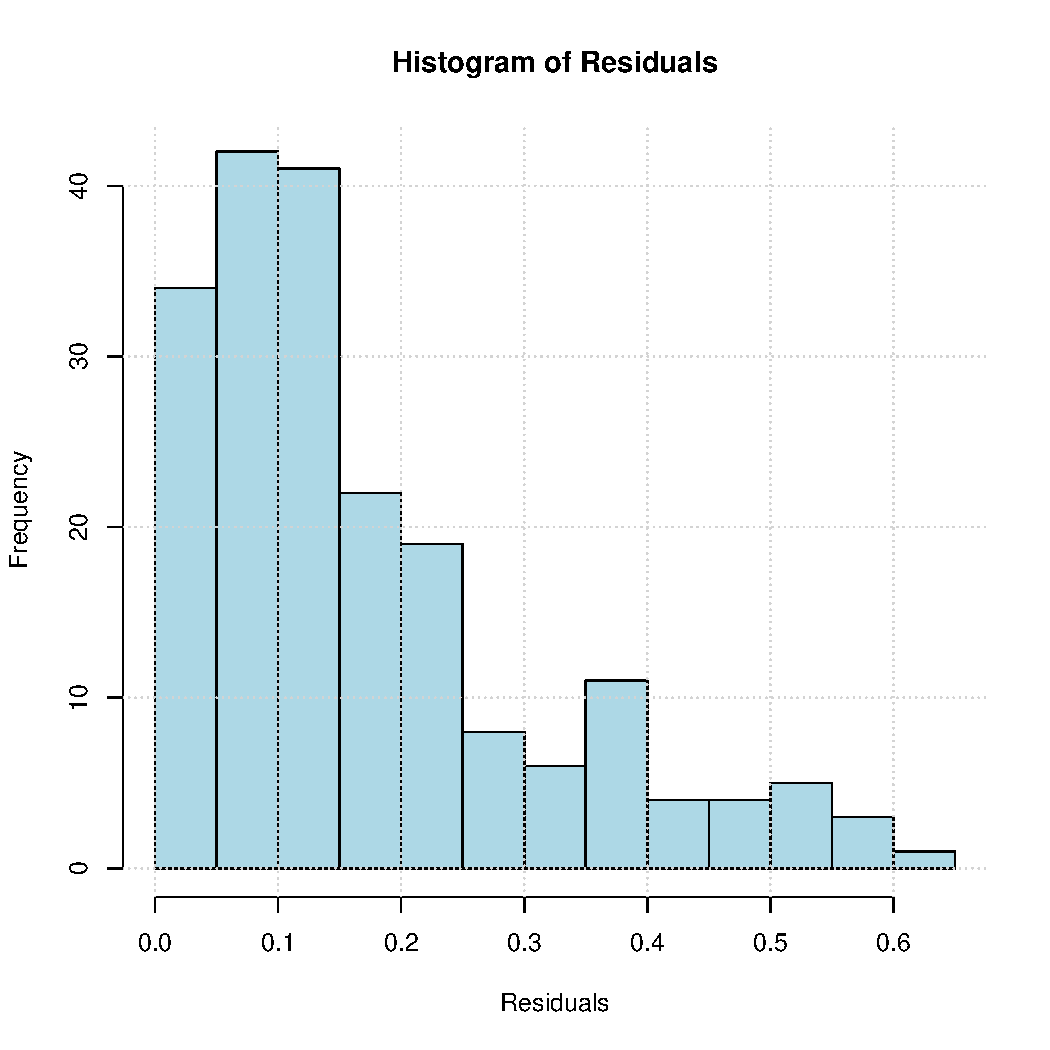
\includegraphics[width=\linewidth]{Images/Figures_Exercise_5/Residual_histo.pdf} 
  \caption{Freq - Historgram, residuals}
  \label{fig:histogram}
\end{subfigure}
\caption{Various plots of accuracy measurements}
\label{fig:three_images}
\end{figure}
\nssection{c.)}
\emph{Discuss the choices made and comment on the results from b.} \spaze
\textbf{Solution:} \spaze
The results in (b.) show clear promise of an architecture that yield both feasible and decent estimates. We can be assured that for the given data, and presumably data structured simirlaly in 1D, the network will provide an "accurate" \footnote{Accurate is in every sense of its meaning interpreted loosely, especially in statistics, but one might be advised to understand it in this particular instance as a precise regression estimate.} description of its reality. But there are naturally a few catches to elaborate on. \spaze 
Having a neural network with only one layer of 50 nodes (or any number of nodes $> 1$) may not be advised for several reasons. Firstly, the complexity of many real-world problems often require more than one layer to capture the intricate and oftentimes stochastic patterns in the data effectively. A single layer might not have enough capacity to learn complex relationships between inputs and outputs. Additionally, a larger number of nodes in a single layer can lead to overfitting, where the network memorizes the training data instead of learning how to generalise patterns, especially if the dataset is not sufficiently large or sparse. \spaze 
The ReLU activation function, while being simplistic and capable of diminishing the vanishing gradient problem, may not always be the best choice. Its main limitation is the "dying ReLU" problem, where neurons can become inactive during training. Furthermore, ReLU lacks a bounded output range, which can also lead to exploding activations. It is not suitable for models requiring negative activations, such as some generative models. Alternative functions like Leaky ReLU or ELU might be better in such cases. In general, for overall performance in a neural network, functions like ADAM, $\tanh$, Sigmoid and RMSprop might be preffered. \spaze 
Lastly, a neural network's sensitivity to learning rate comes from its crucial role in controlling the size of parameter updates during training. If the learning rate is too high, the network may fail to converge or oscillate. Conversely, if it is too low, convergence might be slow. Thus, selecting an optimal learning rate is vital for stable and efficient training. In this respective example we observed the prominent sensitivity which the model had towards its parameters during training, notably for higher learning rates. It was found that on many occasions the gradients would simply explode due to the instability of the hyper-parameters which led to more meticulous grid-searches on the optimal balance between inital learning rate and learning rate decay.